% !TEX program = xelatex
% DeepMimic author-hosted TOG2018 PDF, Sections3-7/9 and AppendixA-D.
% Hybrid diagram. Original imagegen-draft 1024x1536 at72dpi retained unchanged.
% Graphic crops listed here are illustrations only; all causal arrows/math are editable.
\documentclass[tikz,border=0bp]{standalone}
\usepackage{lmodern,fontspec,xeCJK,amsmath,amssymb,graphicx}
\setsansfont{Arial}
\setCJKmainfont[Path=/System/Library/Fonts/,BoldFont={STHeiti Medium.ttc}]{STHeiti Light.ttc}
\setCJKsansfont[Path=/System/Library/Fonts/,BoldFont={STHeiti Medium.ttc}]{STHeiti Light.ttc}
\renewcommand{\familydefault}{\sfdefault}
\usetikzlibrary{arrows.meta,calc}
\definecolor{ink}{HTML}{173646}\definecolor{teal}{HTML}{167D81}\definecolor{amber}{HTML}{A45D18}\definecolor{coral}{HTML}{D95C47}\definecolor{pale}{HTML}{F2F8F7}\definecolor{warm}{HTML}{FFF7E9}\definecolor{navy}{HTML}{314976}\definecolor{blue}{HTML}{F2F5FB}
\tikzset{txt/.style={text=ink,font=\fontsize{14}{18}\selectfont,align=center,inner sep=0},hd/.style={txt,font=\bfseries\fontsize{17}{21}\selectfont},sm/.style={txt,font=\fontsize{13}{17}\selectfont},a/.style={-{Stealth[length=5bp,width=4bp]},line width=1.3bp,draw=teal,rounded corners=3bp},train/.style={a,draw=coral,dashed},box/.style={rounded corners=8bp,line width=.9bp}}
\newcommand{\txt}[4]{\node[txt,text width=#3bp]at(#1,#2){#4};}
\newcommand{\smalltxt}[4]{\node[sm,text width=#3bp]at(#1,#2){#4};}
\newcommand{\head}[4]{\node[hd,text width=#3bp]at(#1,#2){#4};}
\newcommand{\panel}[5]{\draw[box,draw=#4!55,fill=#5](15,#1)rectangle(325,#2);\node[hd,anchor=west,text=#4]at(27,#1+22){#3};}
\newcommand{\art}[7]{\begingroup\pgfmathsetmacro{\bt}{1536-#2-#4}\pgfmathsetmacro{\rt}{1024-#1-#3}\node[anchor=north west,inner sep=0]at(#5,#6){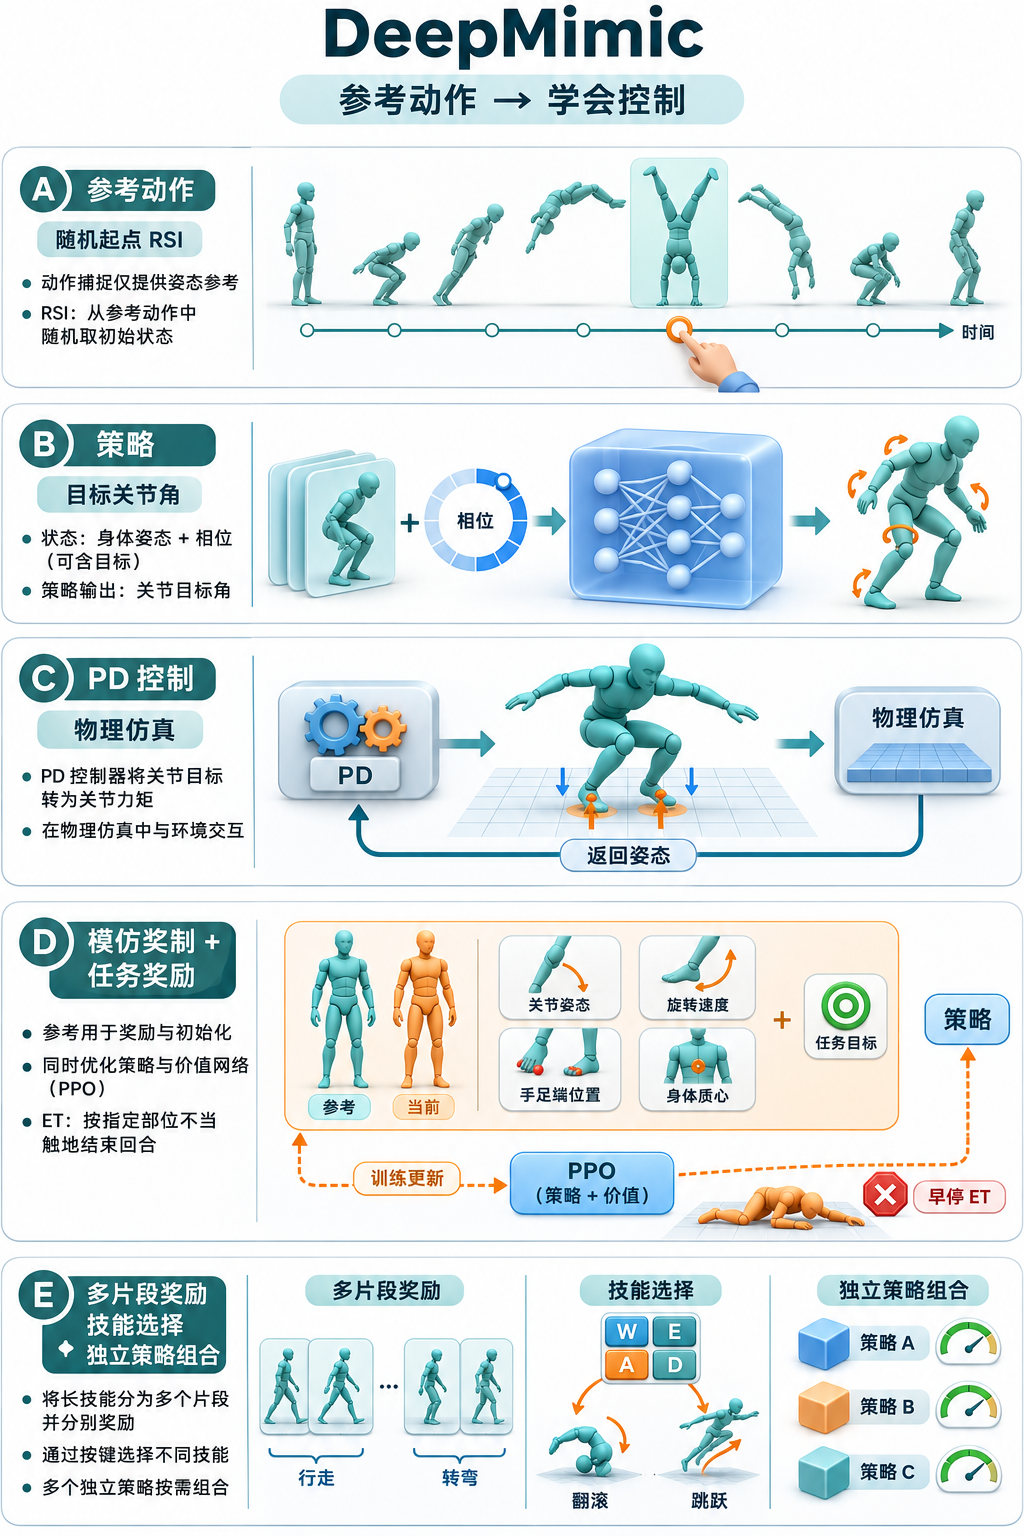
\includegraphics[trim=#1bp \bt bp \rt bp #2bp,clip,width=#7bp]{deepmimic-imagegen-draft.png}};\endgroup}
\begin{document}\begin{tikzpicture}[x=1bp,y=-1bp]
\path[use as bounding box](0,0)rectangle(340,1740);\fill[white](0,0)rectangle(340,1740);
\head{170}{19}{330}{DeepMimic：照着做，还得站得稳}
\smalltxt{170}{47}{320}{青色实线：运行数据\quad 橙色虚线：训练}
\panel{68}{267}{A\quad 参考动作给起点和标准}{teal}{pale}
\art{263}{156}{742}{236}{24}{107}{291}
\txt{170}{218}{290}{RSI：从参考片段随机取完整初态}
\smalltxt{170}{239}{288}{姿态、速度、相位初始化 C 的角色}
\smalltxt{170}{257}{288}{同一参考片段供 D 比较，参与奖励}
% Reference initialization branch to physics state; not a per-step reference input to policy.
% RSI route stated explicitly in A footer; reference never enters runtime policy as a target pose.
\panel{288}{598}{B\quad 当前状态算出关节目标}{navy}{blue}
\art{269}{452}{137}{151}{29}{334}{65}
\art{566}{424}{223}{185}{127}{329}{86}
\art{837}{412}{165}{200}{244}{330}{66}
\draw[a](94,373)--(115,373);\draw[a](222,373)--(239,373);
\smalltxt{64}{430}{88}{本体状态 $s_t$\\含相位 $\phi_t$}
\smalltxt{169}{430}{110}{策略 $\pi_\theta$\\目标 $g_t$ 可选}
\smalltxt{274}{430}{91}{动作 $a_t$\\关节目标角}
\smalltxt{170}{461}{290}{Humanoid（无额外目标或地形输入）}
\txt{170}{484}{290}{$197\to1024\to512\to36$}
\smalltxt{170}{507}{288}{中间层 ReLU，最后一层线性输出均值}
\txt{170}{534}{290}{$\pi_\theta(a_t\mid s_t,g_t)=\mathcal N(\mu_\theta,\Sigma)$}
\smalltxt{170}{559}{290}{$\Sigma$ 固定且对角；训练时按分布采样}
\smalltxt{170}{582}{290}{地形任务：$H\to\mathrm{CNN}\to64$维，再拼接}
\draw[a](170,598)--(170,618);
\panel{621}{847}{C\quad PD 把目标变成力矩}{teal}{pale}
\art{276}{678}{166}{124}{27}{668}{84}
\art{449}{643}{344}{188}{152}{661}{164}
\draw[a](112,708)--(150,708);\smalltxt{131}{684}{39}{$\tau_t$}
\smalltxt{69}{750}{92}{稳定 PD\\局部反馈}
\smalltxt{231}{765}{170}{Bullet 物理仿真\\含接触与重力}
\txt{170}{808}{288}{策略 30 Hz\quad 物理仿真 1.2 kHz}
\smalltxt{170}{832}{288}{得到 $s_{t+1}$，下一控制步回到 B}
\draw[a](325,750)--(334,750)--(334,326)--(64,326)--(64,333);
% Runtime state-feedback arrow is explained in C footer.
\panel{872}{1317}{D\quad 用奖励与回报训练网络}{amber}{warm}
\art{300}{928}{175}{195}{28}{919}{84}
\art{493}{930}{264}{185}{155}{922}{153}
\smalltxt{69}{1036}{90}{参考与当前}
\smalltxt{233}{1036}{167}{姿态／速度／手足／质心}
\txt{170}{1072}{290}{$r_t^I=0.65r_t^p+0.10r_t^v$}
\txt{170}{1096}{290}{$\hphantom{r_t^I=}+0.15r_t^e+0.10r_t^c$}
\txt{170}{1128}{290}{有任务：$r_t=0.7r_t^I+0.3r_t^G$}
\smalltxt{170}{1157}{288}{ET：指定部位不当触地，终止并余奖归零}
\draw[train](170,1173)--(170,1193);
\draw[box,fill=white,draw=amber!60](30,1197)rectangle(310,1300);
\head{170}{1218}{270}{轨迹批次 $\to$ PPO + 价值学习}
\smalltxt{170}{1247}{270}{GAE$(\lambda)$ 优势 $\to$ 更新 B 的策略 $\theta$}
\smalltxt{170}{1273}{270}{TD$(\lambda)$ 目标 $\to$ 更新价值 $\psi$}
% Actual training update path terminates at the policy network, not its inputs.
% Update destination B stated next to the update equation to avoid a crossing through the B title.
% Physics transition feeds the train batch, distinct from the runtime feedback.
\draw[train](325,789)--(334,789)--(334,1218)--(310,1218);
% Orange route carries simulator transitions to the training batch.
% Reference-to-reward path avoids policy runtime path.
% Reference source is identified by the A footer and by the reference/current illustrations in D.
\panel{1342}{1725}{E\quad 三种技能组织方式}{navy}{blue}
\smalltxt{170}{1385}{290}{三条并列选择；各有不同训练与调用方式}
\art{257}{1335}{267}{123}{30}{1415}{99}
\txt{226}{1432}{169}{相似片段，取最高奖励}
\smalltxt{226}{1461}{170}{$r_t^I=\max_j r_t^j$，训练一个策略}
\draw[draw=navy!20](29,1490)--(310,1490);
\art{548}{1320}{202}{155}{30}{1507}{99}
\txt{226}{1529}{170}{one-hot 指定技能}
\smalltxt{226}{1558}{169}{$g_t=\mathbf e_i$，只比较第 $i$ 段}
\draw[draw=navy!20](29,1601)--(310,1601);
\art{792}{1314}{208}{185}{30}{1613}{97}
\txt{226}{1641}{170}{独立训练，再按价值选择}
\smalltxt{226}{1670}{169}{$p^i(s)\propto e^{\bar V^i(s)/\mathcal T}$}
\smalltxt{170}{1707}{288}{周期边界抽一个技能，执行完整周期}
\end{tikzpicture}\end{document}
